\documentclass{beamer}
\usetheme{Frankfurt}
\usecolortheme{seahorse}
\title{Parsing Expression Grammars}
\author{Niccolò Piazzesi}
\institute[UniPi]{
    Università degli Studi di Pisa \\
    Anno Accademico 2020-21
}
\setbeamertemplate{bibliography item}{\insertbiblabel}
\beamertemplatenavigationsymbolsempty
\setbeamertemplate{footline}[page number]
\AtBeginSection[]{
  \begin{frame}
  \vfill
  \centering
  \begin{beamercolorbox}[sep=8pt,center,shadow=true,rounded=true]{title}
    \usebeamerfont{title}\insertsectionhead\par%
  \end{beamercolorbox}
  \vfill
  \end{frame}
}

\begin{document}
    \begin{frame}
        \maketitle
    \end{frame}
    \section{Parsing}
\begin{frame}
    \begin{block}{What's a parser?}
        Part of the compiler.
        Checks the stream of tokens produced by the \emph{lexer} for syntactical errors
        and produces an IR representation (usually an abstract syntax tree) of the source 
        that is used in later steps to generate machine code.
    \end{block}
    \begin{figure}
        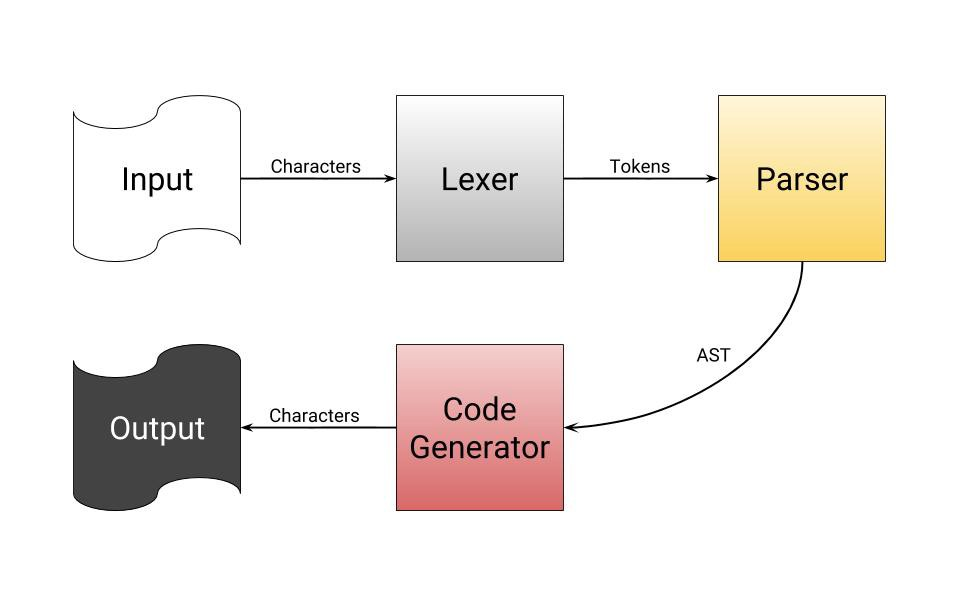
\includegraphics[width=\textwidth]{img/parser.jpg}
    \end{figure}
\end{frame}
\begin{frame}
    \frametitle{Context free grammars}
    
    \begin{block}{}We need a model to describe a language syntax.\end{block}
    \pause
    \begin{block}{}Classical problem, solved by using formal language theory.\end{block}
    \pause
    \begin{block}{}{Syntax described by a \textbf{Context Free Grammar}.}\end{block}

\end{frame}
\begin{frame}
    \frametitle{CFG: definition}
    Context free grammar defined as:
    \begin{center}
        \textbf{G = (V,$\Sigma$, P, S)}
    \end{center}
    \begin{itemize}
        \item V = variables
        \item $\Sigma$ = terminals
        \item P = productions (or rules)
        \item S = start variables
    \end{itemize}
    Productions are in the form A $\rightarrow \alpha$, where A$\in$ V, $\alpha \in (V \cup \Sigma)$

    S $\Rightarrow$ A $|$ bb
    
    A $\Rightarrow$ B $|$ b 
   
    B $\Rightarrow$ S $|$ a
\end{frame}
\begin{frame}
    
        \begin{block}{}
        Given the rules of grammar G, we want to find a sequence of productions that 
        generates a target expression (\textbf{derivation}).
    
        
        \end{block}
        \begin{block}{}
        Parsing is the process of discovering such sequence.
        \end{block}
        
        $ S \rightarrow \gamma_{1} \rightarrow \gamma_{2} \rightarrow \dots \rightarrow \gamma_{n} \rightarrow expression$
        
        \begin{block}{}\textbf{Leftmost derivation}: at each step expand the leftmost non-terminal symbol\end{block}
        
        \begin{block}{}\textbf{Rightmost derivation}: at each step expand the rightmost non-terminal symbol\end{block}
        
\end{frame}
\begin{frame}
   \begin{columns}
       \begin{column}{0.4\textwidth}
           \begin{figure}
               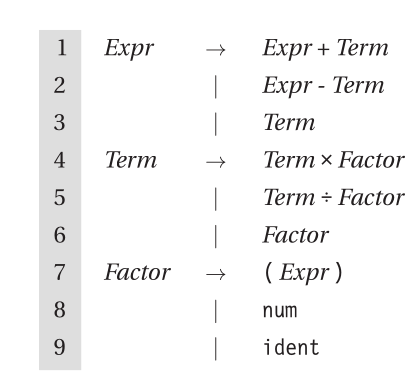
\includegraphics[width=\textwidth]{img/cfg.png}
               \caption{classic grammar for arithmetic expressions}
           \end{figure}
       \end{column}
       \begin{column}{0.6\textwidth}
        \begin{figure}
            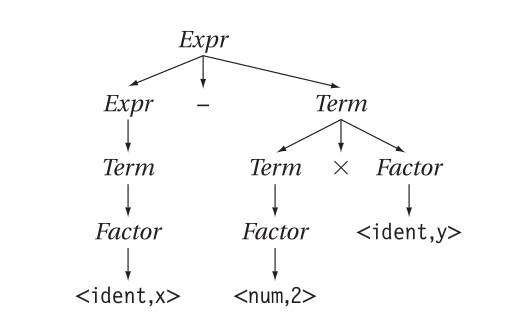
\includegraphics[width=\textwidth]{img/parse.png}
            \caption{parse tree for the expression x-2*y}
        \end{figure}
           
       \end{column}
   \end{columns}
\end{frame}
\begin{frame}
    \frametitle{Parsing techniques}
    Two main techniques:
    \begin{itemize}
        \item Top Down (recursive descent)
        
        Builds the parse tree from root to leaves. 
        Can be modified to do predicitve parsing (LL(1) parser).
        \item Bottom Up
        
        LR(1) parsers, build the parse tree from leaves to root. Bottom-up parsing handles a larger set of
        grammars
    \end{itemize}
   
    \textbf{We will focus on top down parsers.}
\end{frame}
\begin{frame}
    \frametitle{Top down parsers}
    \begin{block}{}Start from root of parse tree \end{block}
    \begin{block}{}At each level pick a production to match the input\end{block}
    \begin{block}{}If the derivation doesn't match the input $\Rightarrow$ backtrack and pick a different production\end{block}
\end{frame}
    \section{PEG: Definition and main features}
\begin{frame}
    \frametitle{Formal definition \cite{peg}}
\end{frame}
    \section{A use case: \emph{pgen}}
\begin{frame}
    While being a relatively new subject, parsing expression grammars have recently proved their  power in concrete parsers implementation.
    
    \begin{block}{}
    	In PEP 617 \cite{python}, CPython creator and mantainer Guido Van Rossum announced the proposal of replacing the old python parser generator, named pgen, with a new PEG parser generator.
    \end{block}
	\begin{block}{}
		The proposal has been accepted, and the new module has been introduced in python 3.9. The old parser will still be the main Python parser until version 3.10, where it will be completely replaced.
	\end{block}
\end{frame}

\begin{frame}[fragile]
	\small
	\frametitle{Python parser: an overview}
	Despite technically being LL(1), the Python grammar have several rules that are not LL(1), requiring several workarounds to be used in the grammar and other parts of CPython.  

		Sometimes the problem is not solvable with any workaround. As an example, no LL(1) rule can be made to support writing multiline parenthesized context managers:
		\begin{minted}{Python}
		with(
		open("a") as a,
		open("b") as b,
		open("c") as c,
		)
		\end{minted}

Since open parenthesis are in the first sets of grammar items that can appear as context managers, the rule would be ambigous.
\end{frame}

\begin{frame}
	\frametitle{Other issues}
	\begin{itemize}
		\item Huge coupling between AST generation routines and the shape of the resulting tree. Many actions are directly tied to the implicit structure of the ast, making the code more complex and implementation dependent.
		\item No left recursion allowed, since the grammar is LL(1).
		
		\item The current parser does not directly generate the AST. It instead creates a Concrete Syntax Tree, which is then  transformed to an abstract one. This structure is not used by anything else and it requires to be kept entirely in memory, heavily  increasing space consumption.
	\end{itemize}
\end{frame}

\begin{frame}
	\frametitle{The proposal}
	The new proposed PEG parser is divided in three components:\begin{enumerate}
		\item A parser generator. It reads  a grammar file and produces a PEG parser written in Python or C.
		
		\item A PEG meta-grammar that auto generates a Python parser used for the parser generator itself
		\item A generated parser that produces C and Python AST objects.
	\end{enumerate} 
\end{frame}
\begin{frame}
	\frametitle{Features}
	
	\begin{block}{Left recursion}
		While PEG parsers normally do not support it, the proposed parser can handle both direct and indirect left recursion, thanks to a memoization cache.
	\end{block}

	\begin{block}{Syntax}
		The syntax is quite similar to the one that we saw. For simplicity the left arrow $\leftarrow$ is replaced by ' : ' and the choice operator reuses the symbol ' $|$ '.
	\end{block}

	\begin{block}{Grammar actions}
		The proposed PEG parser is able to directly generate AST nodes  for a rule via grammar actions, which are language specific expressions evaluated when a rule is successfully parsed. This removes the need for an intermediate CST, freeing up space.
	\end{block}


\end{frame}
\begin{frame}
\frametitle{Performance}

During testing, it has been shown that the new parser comes within the performance of the old one up to 10\%, both in time and space consumption.

While the packrat parsing algorithm requires more space of the normal LL(1) parser to store intermediate results, this is balanced by not having to build the intermediate CST.

It has been found that the new parser is slightly faster, but uses around 10\% more memory. 
\end{frame}

\begin{frame}[fragile]
	\huge
	
	Thanks for your attention!
	
	\large 
	\begin{minted}{bash}
>>> __peg_parser__
File "<stdin>", line 1
__peg_parser__
^
SyntaxError: You found it!
\end{minted}

\end{frame}

    \section{Bibliography}
    \begin{frame}[allowframebreaks]
        \frametitle{References}
        \bibliographystyle{abbrv}
        \bibliography{bib.bib}
    \end{frame}
\end{document}